\section{Задание 2.}

\textbf{Условие.}

Найдите первые $k$ членов разложения в степенной ряд решения дифференциального уравнения при указанных 
начальных условиях. 

\begin{gather*}
    y^\prime = x + \arcsin y, \\
    y(0) = 0.5, \ k = 4
\end{gather*}

\vspace{10mm}

\textbf{Решение.}

$y^\prime = x + \arcsin y$

$y(0) = 0.5, \ k = 4$

$y^\prime = 0 + \arcsin y(0) = \arcsin 0.5 = \frac{\pi}{6}$

$y^{\prime\prime} = (x + \arcsin y)^\prime = 1 + \frac{1}{\sqrt{1 - y^2}} \cdot y^\prime$

$y^{\prime\prime}(0) = \frac{2\sqrt{3}}{3} \frac{\pi}{6} + 1 = \frac{\sqrt{3}\pi}{9} + 1$

$y^{\prime\prime\prime} = \left(\frac{1}{\sqrt{1 - y^2}} \cdot y^\prime\right)^\prime = 
\left(\frac{1}{\sqrt{1 - y^2}}\right)^\prime \cdot y^\prime + \frac{1}{\sqrt{1 - y^2}} \cdot y^{\prime\prime} = 
-\frac{1}{2} (1 - y^2)^{-\frac{3}{2}} \cdot (-2y) \cdot (y^\prime)^2 + \frac{1}{\sqrt{1 - y^2}} \cdot y^{\prime\prime}  = 
(1 - y^2)^{-\frac{3}{2}} \cdot y \cdot (y^\prime)^2 + \frac{1}{\sqrt{1 - y^2}} \cdot y^{\prime\prime}
$

$y^{\prime\prime\prime}(0) = \left(\frac{3}{4}\right)^{-\frac{3}{2}} \cdot \frac{1}{2} \cdot \frac{\pi^2}{36} + \frac{2\sqrt{3}}{3} (\frac{\sqrt{3}\pi}{9} + 1) = 
\frac{8}{\sqrt{27}}\frac{\pi^2}{36} + \frac{2\pi}{9} + \frac{2\sqrt{3}}{3} = \frac{\sqrt{3}\pi^2}{81} + \frac{2\pi}{9} + \frac{2\sqrt{3}}{3}$

$y^{(4)} = \left((1 - y^2)^{-\frac{3}{2}} \cdot y \cdot y^\prime + \frac{1}{\sqrt{1 - y^2}} \cdot y^{\prime\prime}\right)^\prime = 
(1 - y^2)^{-\frac{5}{2}} \cdot ((2y^2 + 1) (y^\prime)^3) - (1 - y^2)^{-\frac{3}{2}} \cdot 3y \cdot y^\prime \cdot y^{\prime\prime} + (1 - y^2)^{-\frac{1}{2}} y^{\prime\prime\prime}$

$y^{(4)}(0) = \frac{2\sqrt{3}}{243}\pi^3 + \frac{8}{81}\pi^2 + \frac{10\sqrt{3}}{27} \pi + \frac{4}{3}$

$\displaystyle f(x) = \sum_{n = 0}^4 \frac{f^{(n)}(0)}{n!} x^n = 0.5 + \frac{\pi}{6}x + \left(\frac{\sqrt{3}\pi}{18} + \frac{1}{2}\right){x^2} + \frac{\frac{\sqrt{3}\pi^2}{81} + \frac{2\pi}{9} + \frac{2\sqrt{3}}{3}}{6} x^3 + \frac{\frac{2\sqrt{3}}{243}\pi^3 + \frac{8}{81}\pi^2 + \frac{10\sqrt{3}}{27} \pi + \frac{4}{3}}{24} x^4$

Сравним графики $f^\prime(x)$ и $x + \arcsin(f(x))$:

\begin{center}
    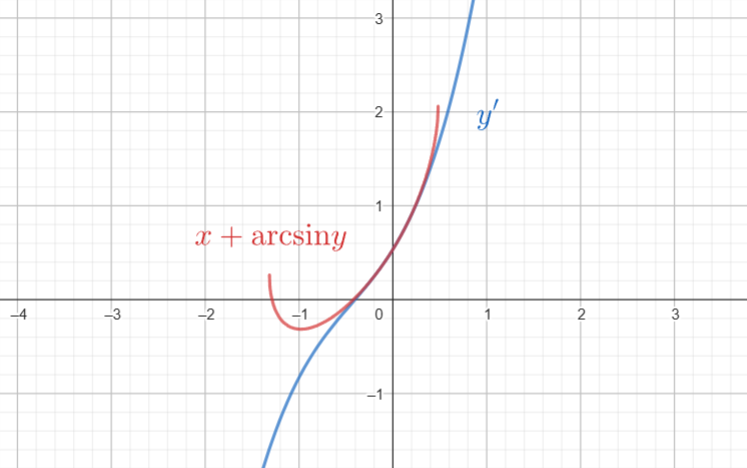
\includegraphics[height=0.45\textwidth]{images/2}
\end{center}

\clearpage
